%  A simple AAU report template.
%  2015-05-08 v. 1.2.0
%  Copyright 2010-2015 by Jesper Kjær Nielsen <jkn@es.aau.dk>
%
%  This is free software: you can redistribute it and/or modify
%  it under the terms of the GNU General Public License as published by
%  the Free Software Foundation, either version 3 of the License, or
%  (at your option) any later version.
%
%  This is distributed in the hope that it will be useful,
%  but WITHOUT ANY WARRANTY; without even the implied warranty of
%  MERCHANTABILITY or FITNESS FOR A PARTICULAR PURPOSE.  See the
%  GNU General Public License for more details.
%
%  You can find the GNU General Public License at <http://www.gnu.org/licenses/>.
%
\usepackage{graphicx,hyperref,amsmath,bm,url}
\usepackage[numbers]{natbib}
\usepackage{microtype,todonotes}
\usepackage[danish]{babel}
\usepackage{a4}
\usepackage[compact,small]{titlesec}
\usepackage[utf8]{inputenc}
\clubpenalty = 10000
\widowpenalty = 10000
\usepackage[T1]{fontenc}
\graphicspath{ {../Billeder/} }
\usepackage{tikz}
\usetikzlibrary{calc}
\usetikzlibrary{shapes}

\makeatletter
\newdimen\@myBoxHeight%
\newdimen\@myBoxDepth%
\newdimen\@myBoxWidth%
\newdimen\@myBoxSize%
\newcommand{\SquareBox}[2][]{%
    \settoheight{\@myBoxHeight}{#2}% Record height of box
    \settodepth{\@myBoxDepth}{#2}% Record depth of box
    \settowidth{\@myBoxWidth}{#2}% Record width of box
    \pgfmathsetlength{\@myBoxSize}{max(\@myBoxWidth,(\@myBoxHeight+\@myBoxDepth))}%
    \tikz \node [shape=rectangle, shape aspect=1,draw=red,inner sep=2\pgflinewidth, minimum size=\@myBoxSize,#1] {#2};%
}%
\makeatother
\newcommand*{\captionsource}[2]{%
  \caption[{#1}]{%
    #1%
    \\\hspace{\linewidth}%
    \textbf{Kilde:} #2%
  }%
}% package inclusion and set up of the document
% see, e.g., http://en.wikibooks.org/wiki/LaTeX/Formatting#Hyphenation
% for more information on word hyphenation
\hyphenation{ex-am-ple hy-phen-a-tion short}
\hyphenation{long la-tex}
% 
%  A simple AAU report template.
%  2015-05-08 v. 1.2.0
%  Copyright 2010-2015 by Jesper Kjær Nielsen <jkn@es.aau.dk>
%
%  This is free software: you can redistribute it and/or modify
%  it under the terms of the GNU General Public License as published by
%  the Free Software Foundation, either version 3 of the License, or
%  (at your option) any later version.
%
%  This is distributed in the hope that it will be useful,
%  but WITHOUT ANY WARRANTY; without even the implied warranty of
%  MERCHANTABILITY or FITNESS FOR A PARTICULAR PURPOSE.  See the
%  GNU General Public License for more details.
%
%  You can find the GNU General Public License at <http://www.gnu.org/licenses/>.
%
%
%
% see, e.g., http://en.wikibooks.org/wiki/LaTeX/Customizing_LaTeX#New_commands
% for more information on how to create macros

%%%%%%%%%%%%%%%%%%%%%%%%%%%%%%%%%%%%%%%%%%%%%%%%
% Macros for the titlepage
%%%%%%%%%%%%%%%%%%%%%%%%%%%%%%%%%%%%%%%%%%%%%%%%
%Creates the aau titlepage
\newcommand{\aautitlepage}[3]{%
  {
    %set up various length
    \ifx\titlepageleftcolumnwidth\undefined
      \newlength{\titlepageleftcolumnwidth}
      \newlength{\titlepagerightcolumnwidth}
    \fi
    \setlength{\titlepageleftcolumnwidth}{0.5\textwidth-\tabcolsep}
    \setlength{\titlepagerightcolumnwidth}{\textwidth-2\tabcolsep-\titlepageleftcolumnwidth}
    %create title page
    \thispagestyle{empty}
    \noindent%
    \begin{tabular}{@{}ll@{}}
      \parbox{\titlepageleftcolumnwidth}{
        \iflanguage{danish}{%
          \includegraphics[width=\titlepageleftcolumnwidth]{aau_logo_da}
        }{%
          
\includegraphics[width=\titlepageleftcolumnwidth]{aau_logo_en}
        }
      } &
      \parbox{\titlepagerightcolumnwidth}{\raggedleft\sf\small
        #2
      }\bigskip\\
       #1 &
      \parbox[t]{\titlepagerightcolumnwidth}{%
      \textbf{Abstract:}\bigskip\par
        \fbox{\parbox{\titlepagerightcolumnwidth-2\fboxsep-2\fboxrule}{%
          #3
        }}
      }\\
    \end{tabular}
    \vfill
    \iflanguage{danish}{%
      \noindent{\footnotesize\emph{Rapportens indhold er frit tilgængeligt, men offentliggørelse (med kildeangivelse) må kun ske efter aftale med forfatterne.}}
    }{%
      \vspace{1mm}\noindent{\footnotesize\emph{The content of this report is freely available, but publication (with reference) may only be pursued due to agreement with the author.}}
    }
    \clearpage
  }
}

%Create english project info
\newcommand{\englishprojectinfo}[8]{%
  \parbox[t]{\titlepageleftcolumnwidth}{
    \textbf{Title:}\\ #1\bigskip\par
    \textbf{Theme:}\\ #2\bigskip\par
    \textbf{Project Period:}\\ #3\bigskip\par
    \textbf{Project Group:}\\ #4\bigskip\par
    \textbf{Participant(s):}\\ #5\bigskip\par
    \textbf{Supervisor(s):}\\ #6\bigskip\par
    \textbf{Copies:} #7\bigskip\par
    \textbf{Page Numbers:} \pageref{LastPage}\bigskip\par
    \textbf{Date of Completion:}\\ #8
  }
}

%Create danish project info
\newcommand{\danishprojectinfo}[8]{%
  \parbox[t]{\titlepageleftcolumnwidth}{
    \textbf{Titel:}\\ #1\bigskip\par
    \textbf{Tema:}\\ #2\bigskip\par
    \textbf{Projektperiode:}\\ #3\bigskip\par
    \textbf{Projektgruppe:}\\ #4\bigskip\par
    \textbf{Deltager(e):}\\ #5\bigskip\par
    \textbf{Vejleder(e):}\\ #6\bigskip\par
    \textbf{Oplagstal:} #7\bigskip\par
    \textbf{Sidetal:} \pageref{LastPage}\bigskip\par
    \textbf{Afleveringsdato:}\\ #8
  }
}

%%%%%%%%%%%%%%%%%%%%%%%%%%%%%%%%%%%%%%%%%%%%%%%%
% An example environment
%%%%%%%%%%%%%%%%%%%%%%%%%%%%%%%%%%%%%%%%%%%%%%%%
\theoremheaderfont{\normalfont\bfseries}
\theorembodyfont{\normalfont}
\theoremstyle{break}
\def\theoremframecommand{{\color{gray!50}\vrule width 5pt \hspace{5pt}}}
\newshadedtheorem{exa}{Example}[chapter]
\newenvironment{example}[1]{%
		\begin{exa}[#1]
}{%
		\end{exa}
}
% my new macros
\usepackage{pdfpages}
\begin{document}
\title{Errata - Hiding in Plain Sight}
\author{DAT2-A423}
\date{30th of June}
\maketitle
\begin{itemize}
\item On page 21 in table 2.2, the DQT marker is wrongly stated to be 0xFFD8. The correct DQT marker is 0xFFDB.

\item On page 22-23 it is stated the encoding of the quantization table values are done top to bottom, left to right. They are however, encoded in a zigzag pattern. 

\item On page 40, figure \ref{fig:WrongJPEGprocess} is shown. The conversion of colour model is from RGB to YCbCr, not from YCbCr to RGB as wrongly stated by the figure. The corrected image can be seen on figure \ref{fig:JPEGprocess}.
\end{itemize}

\begin{figure}
\centering
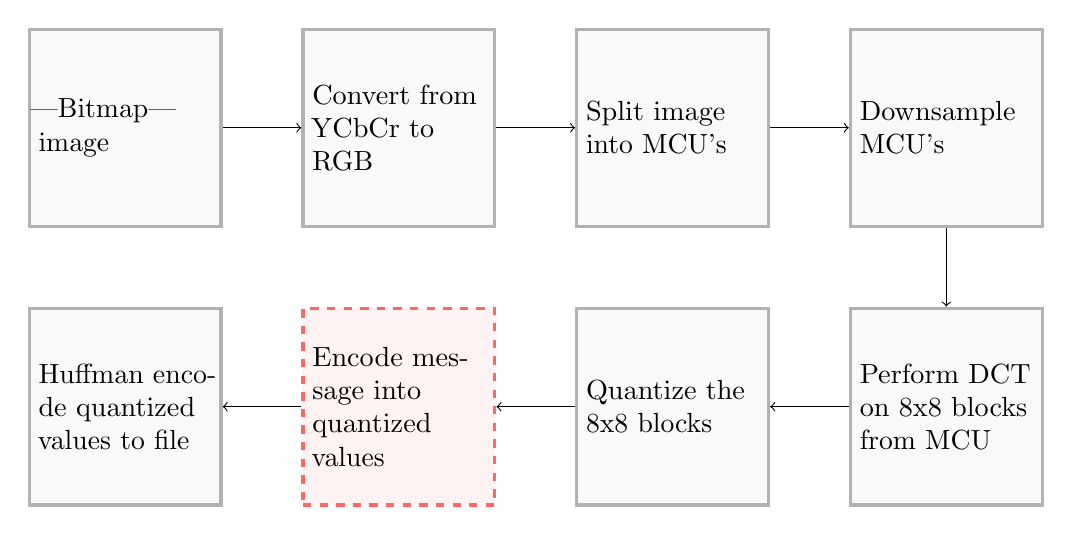
\begin{tikzpicture}[
processnode/.style={rectangle, draw=gray!60, fill=gray!5, very thick, minimum size=5mm,text width=2.2cm, minimum height=2.5cm},
encodenode/.style={rectangle, dashed,draw=red!60, fill=red!5, very thick, minimum size=5mm,text width=2.2cm, minimum height=2.5cm},
pre/.style={=stealth',semithick},
post/.style={->,shorten >=1pt,>=stealth',semithick},
]
%Nodes
\node[processnode]        (huffmanencoding)  {Huffman encode quantized values to file};
\node[encodenode]         (encode)           [right=of huffmanencoding] {Encode message into quantized values};
\node[processnode]        (quantization)     [right=of encode] {Quantize the 8x8 blocks};
\node[processnode]        (dct)              [right=of quantization] {Perform DCT on 8x8 blocks from MCU};
\node[processnode]        (sampling)         [above=of dct] {Downsample MCU's};
\node[processnode]        (split)            [left=of sampling] {Split image into MCU's};
\node[processnode]        (convert)          [left=of split] {Convert from YCbCr to RGB};
\node[processnode]        (bitmapimage)      [left=of convert] {\lstinline|Bitmap| \\image};
 
%Lines
\draw[->] (bitmapimage.east) -- (convert.west);
\draw[->] (convert.east) -- (split.west);
\draw[->] (split.east) -- (sampling.west);
\draw[->] (sampling.south) -- (dct.north);
\draw[->] (dct.west) -- (quantization.east);
\draw[->] (quantization.west) -- (encode.east);
\draw[->] (encode.west) -- (huffmanencoding.east);
\end{tikzpicture}
\caption{Process of encoding a JPEG image with embedding of data}
\label{fig:WrongJPEGprocess}
\end{figure}


\begin{figure}
\centering
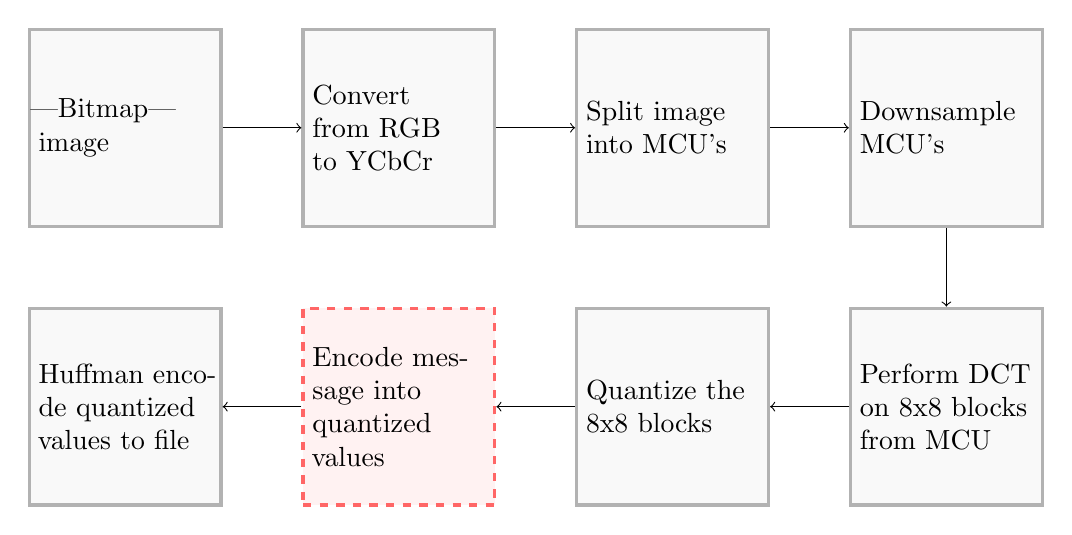
\begin{tikzpicture}[
processnode/.style={rectangle, draw=gray!60, fill=gray!5, very thick, minimum size=5mm,text width=2.2cm, minimum height=2.5cm},
encodenode/.style={rectangle, dashed,draw=red!60, fill=red!5, very thick, minimum size=5mm,text width=2.2cm, minimum height=2.5cm},
pre/.style={=stealth',semithick},
post/.style={->,shorten >=1pt,>=stealth',semithick},
]
%Nodes
\node[processnode]        (huffmanencoding)  {Huffman encode quantized values to file};
\node[encodenode]         (encode)           [right=of huffmanencoding] {Encode message into quantized values};
\node[processnode]        (quantization)     [right=of encode] {Quantize the 8x8 blocks};
\node[processnode]        (dct)              [right=of quantization] {Perform DCT on 8x8 blocks from MCU};
\node[processnode]        (sampling)         [above=of dct] {Downsample MCU's};
\node[processnode]        (split)            [left=of sampling] {Split image into MCU's};
\node[processnode]        (convert)          [left=of split] {Convert from RGB to YCbCr};
\node[processnode]        (bitmapimage)      [left=of convert] {\lstinline|Bitmap| \\image};
 
%Lines
\draw[->] (bitmapimage.east) -- (convert.west);
\draw[->] (convert.east) -- (split.west);
\draw[->] (split.east) -- (sampling.west);
\draw[->] (sampling.south) -- (dct.north);
\draw[->] (dct.west) -- (quantization.east);
\draw[->] (quantization.west) -- (encode.east);
\draw[->] (encode.west) -- (huffmanencoding.east);
\end{tikzpicture}
\caption{Process of encoding a JPEG image with embedding of data}
\label{fig:JPEGprocess}
\end{figure}



\end{document}